
\begin{frame}
\titlepage % Print the title page as the first slide
\end{frame}






\section{Motivation} 


\begin{frame}[label=motivatingslide]
\frametitle{Motivating Slide }
\begin{figure}[H]  %for putting in a single figure
\center{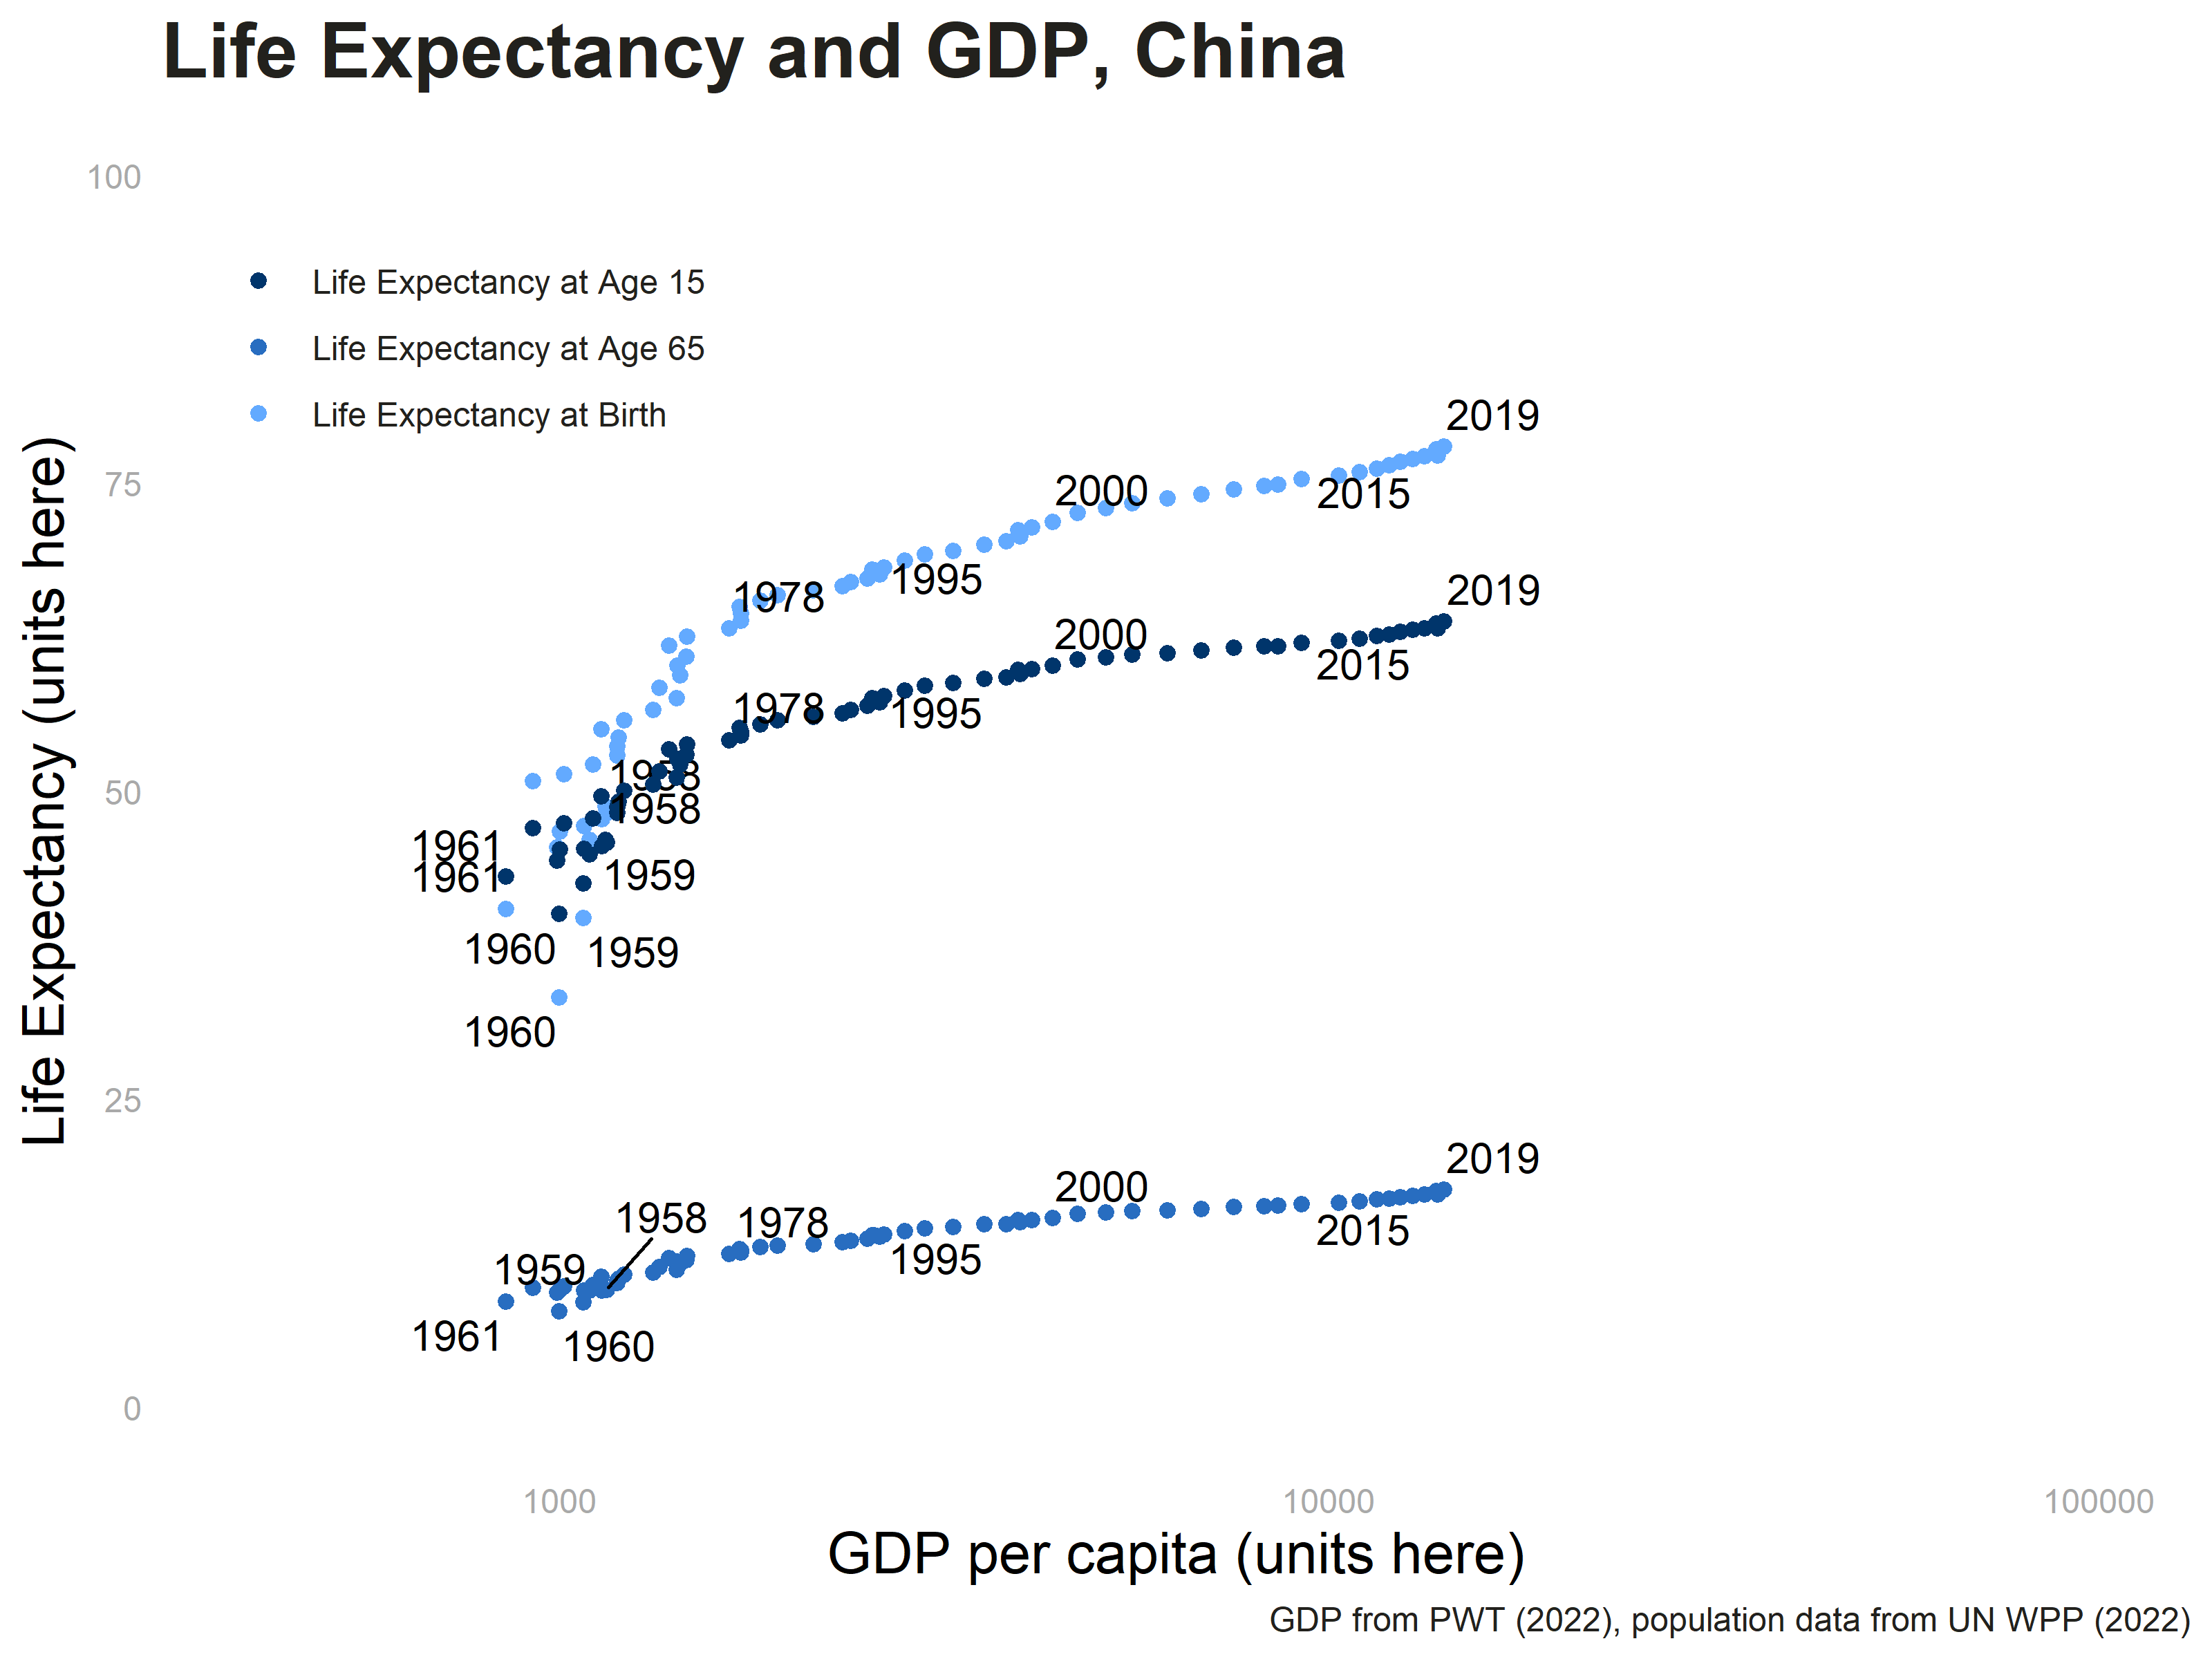
\includegraphics[width=.4\linewidth]{figures/ECON-412/gdp_pc_le_China.png}}\\
{\tiny Female - Male Life Expectancy\\
BrickRed - females vulnerable; green - neutral; yellow - males vulnerable}
\tiny{(Picture source: Woman Stats, 2013 Data)}
\label{fig:speciation}
\end{figure}
\end{frame}


\begin{frame}[label = pictransition]
\frametitle{Transitioning between pictures on a slide }
\begin{figure}
    \begin{center}
\includegraphics<1>[width=.7\linewidth]{figures/ECON-412/gdp_pc_le_1950.png}
\includegraphics<2>[width=.7\linewidth]{figures/ECON-412/gdp_pc_le_2019.png}
\\
{\tiny Green - parity; Hotter - worse for females.\\
Data source: 10\% Census, China Statistical Bureau, (Lai 2004)\\
Created by the author in GIS}
    \end{center}
\end{figure}
\end{frame}


\begin{frame}
\frametitle{Single Picture on a Slide}
\begin{figure}[H]  %for putting in a single figure
\center{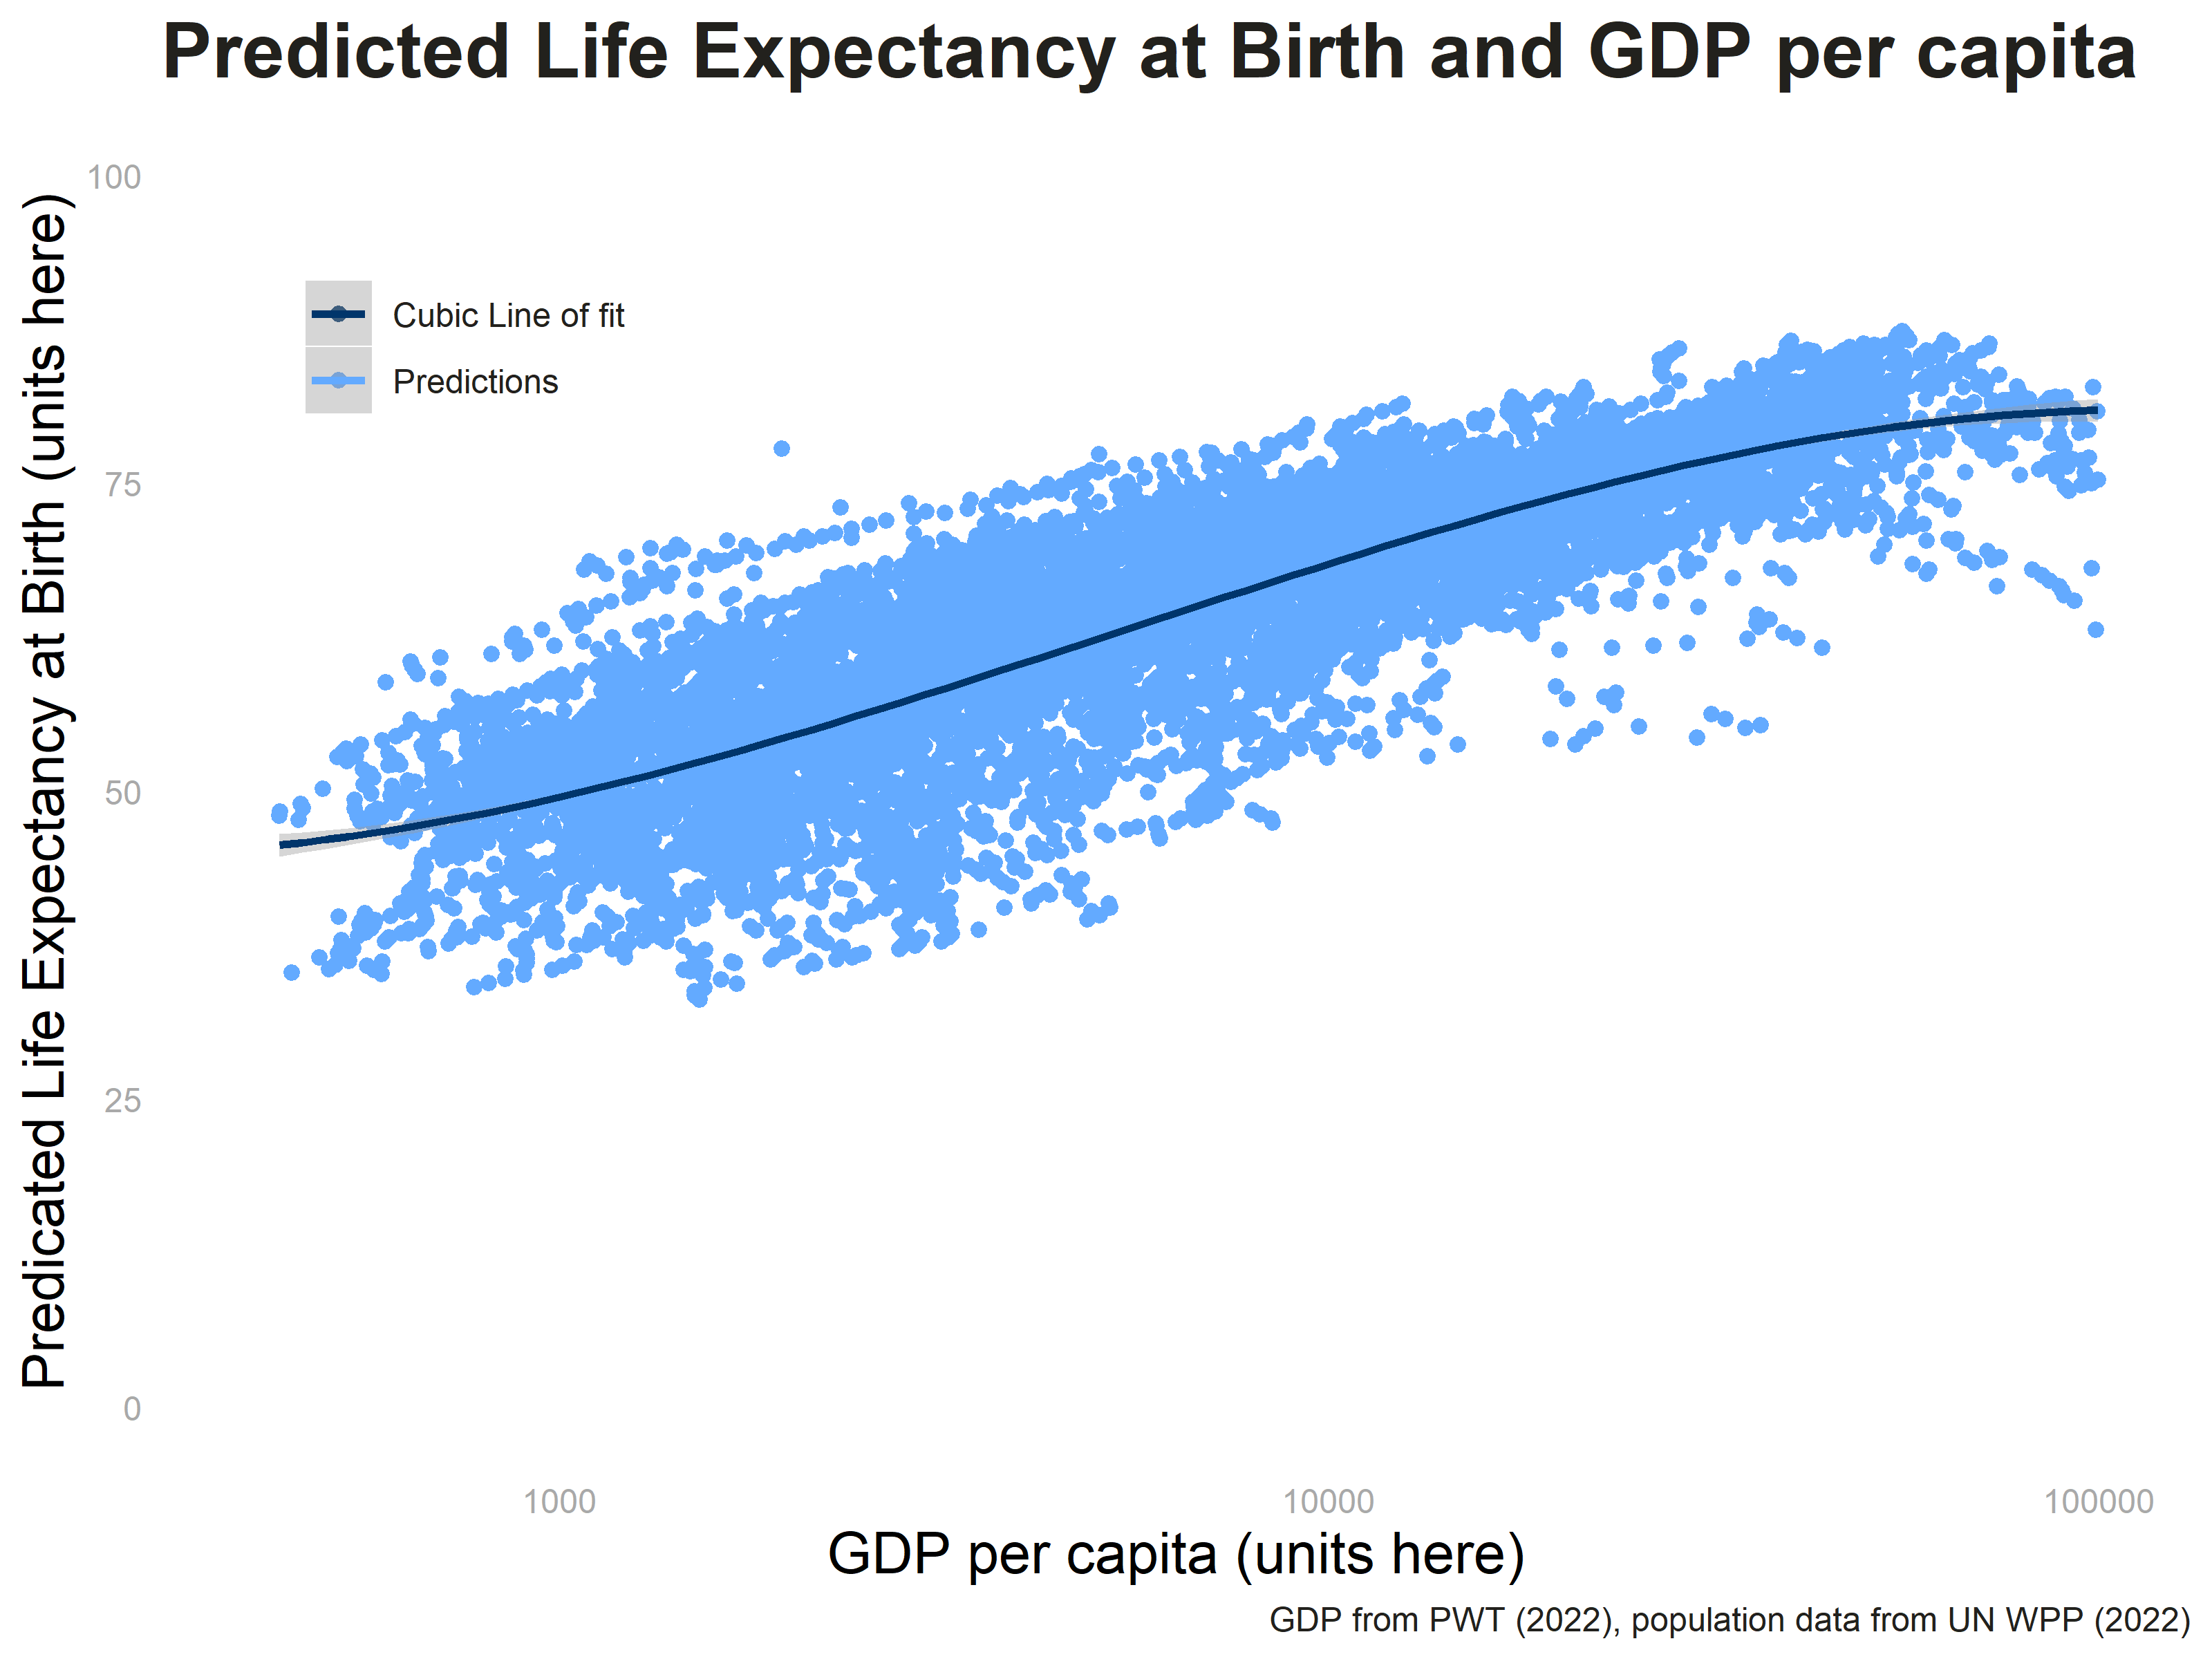
\includegraphics[width=.6\linewidth]{figures/ECON-412/gdp_pc_le_predictions.png}}
\caption{Caption\\
\bigskip
\small{(Picture source ())}}
\end{figure}
\end{frame}

\section{Introduction}

\begin{frame}
\frametitle{Lists with Pauses}

\begin{itemize}
\item - Thing Ar
\begin{itemize}
\item item
\end{itemize}
\pause
\item - Thing B
\begin{itemize}
\item - item
\end{itemize}
\pause
\item - Thing C
\end{itemize}
\end{frame}


\end{frame}



\begin{frame}[label=contracts]
\frametitle{Complicated Slide Patterns}


\only<1,2>{
Consequences for reneging
\begin{itemize}
    \item 1) Loss of future insurance (for $p$ periods)
    \item 2) Direct penalty if $i$ breaches in state $s$:
    \[P_i(s) \geq 0\]
\end{itemize}

}

\only<1>{
\begin{figure}
    \begin{center}

\includegraphics[width=.4\linewidth]{figures/did-best-no-regrets.png}
\caption{\href{https://image.baidu.com/search/detail?ct=503316480&z=undefined&tn=baiduimagedetail&ipn=d&word=\%E5\%BD\%9D\%E6\%97\%8F\%E8\%80\%81\%E5\%A5\%B6\%E5\%A5\%B6&step_word=&ie=utf-8&in=&cl=2&lm=-1&st=undefined&hd=undefined&latest=undefined&copyright=undefined&cs=3085918882,1794597568&os=2121881709,435041436&simid=3410413791,324683210&pn=23&rn=1&di=2970&ln=669&fr=&fmq=1638904755920_R&fm=&ic=undefined&s=undefined&se=&sme=&tab=0&width=undefined&height=undefined&face=undefined&is=0,0&istype=0&ist=&jit=&bdtype=0&spn=0&pi=0&gsm=0&objurl=https\%3A\%2F\%2Fgimg2.baidu.com\%2Fimage_search\%2Fsrc\%3Dhttp\%253A\%252F\%252Fimg.mala.cn\%252Fforum\%252F201208\%252F21\%252F184006422u3auui2prmu52.jpg\%26refer\%3Dhttp\%253A\%252F\%252Fimg.mala.cn\%26app\%3D2002\%26size\%3Df9999\%2C10000\%26q\%3Da80\%26n\%3D0\%26g\%3D0n\%26fmt\%3Djpeg\%3Fsec\%3D1641496752\%26t\%3Df138f1b4a274699e8d714b6bf0011db8&rpstart=0&rpnum=0&adpicid=0&nojc=undefined&dyTabStr=MCwzLDQsNiwxLDUsMiw3LDgsOQ\%3D\%3D}{(Source: Baidu)}}
\end{center}
\end{figure}
}

\only<2>{
\begin{itemize}
    \item - For $P_i(s)$ large enough, full insurance
    \item - If $\delta$ and $P_i(s)$ small enough, autarky
    \item - Focus on the middle cases, partial insurance
\end{itemize}
}

\only<3>{
For $s_t$ the state in time $t$, define
\begin{itemize}
    \item - Contract $\tau(\cdot)$ for each $t$ and each history $h_t = (s_1,s_t,\ldots,s_t)$
    \item - Defines transfer $\tau(h_t)$ from HH1 to HH2 
    \item - {\footnotesize ($\tau(h_t)<0$ is a transfer from HH2 to HH1)}
    \item - {\footnotesize $h_{t-1} = \varnothing$ for $t=1$}
\end{itemize}

}

\only<4>{
Define $U_t(h_t)$ as the expected utility gain over autarky (surplus) for HH1 under contract $\tau$, history $h_t$:
}

\only<4,5,6>{
\begin{equation}
    \begin{split}
       U_t (h_t )& =\\
       & u(y_1 (s_t ) - \tau(h_t )) - u(y_1 (s_t ))+ \quad \text{(SR gain)}\\
       & \mathbb{E}\left[\sum_{j=t+1}^{\infty}\left[\delta^{j-t} [u(y_1 (s_j )- \tau(h_j ))- u(y_1 (s_j ))\right]\right]  \quad \text{(LR gain)}
    \end{split}
\end{equation}
}

\only<4>{
Ditto $V_t(h_t)$ for HH2.
}

\only<5,6>{
Sustainability Constraints: 

\begin{equation}
    U_t(h_t) \geq -P_1(s_t)
\end{equation}

\begin{equation}
    V_t(h_t) \geq -P_2(s_t)
\end{equation}


}

\only<6>{

What's the interpretation of these?

}


\end{frame}



\begin{frame}
\frametitle{Overview} % Table of contents slide, comment this block out to remove it
\tableofcontents % Throughout your presentation, if you choose to use \section{} and \subsection{} commands, these will automatically be printed on this slide as an overview of your presentation
\end{frame}



\section{Background}



\begin{frame}[label = source-slide]
\frametitle{Source slide \hyperlink{data}{\beamerbutton{Back to Data}}}
\begin{figure}
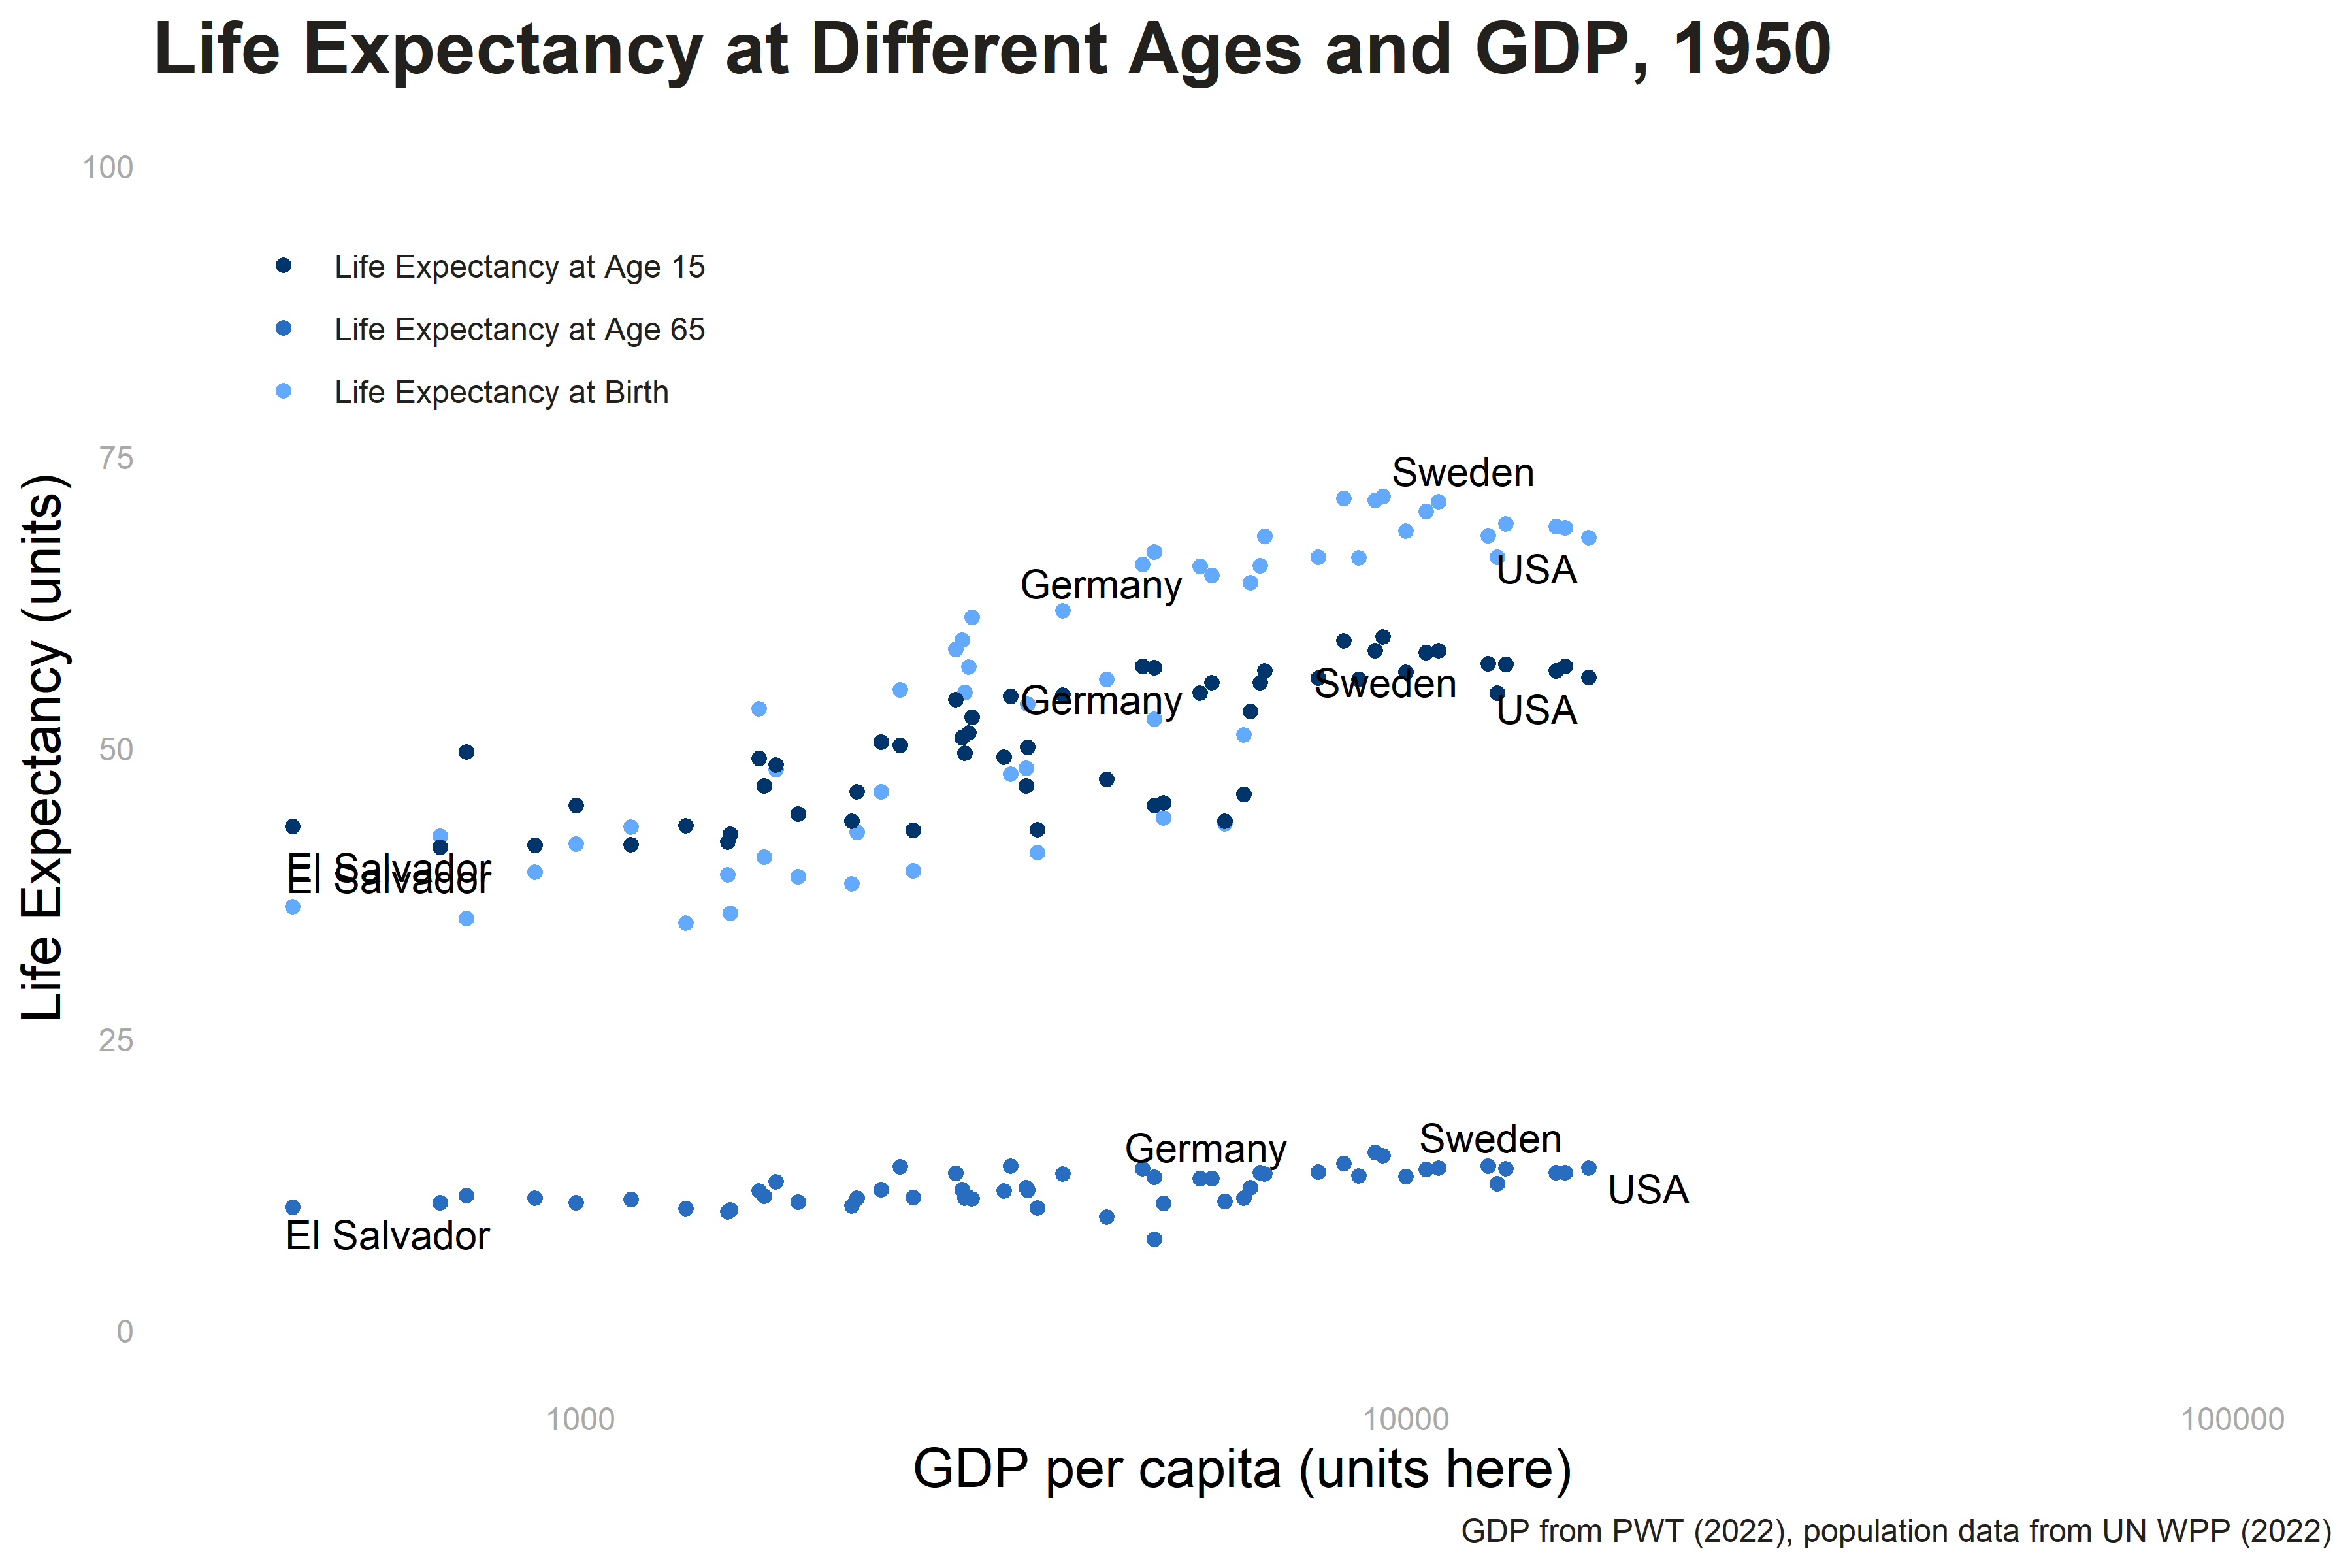
\includegraphics[width=.5\textwidth]{figures/ECON-412/gdp_pc_le_1950.png} \vspace*{-.5cm}\\%\hspace*{2cm} \\
\end{figure}
\begin{itemize}
\item - Mostly (over 90\%) agrarian
\item - Treaty of Tianjin opened Yingkou to trade in 1861
\end{itemize}
\hyperlink{target-slide}{\beamerbutton{Target Slide}}
\end{frame} 


\begin{frame}{Side by side images in Beamer}{Bottom vertical alignment}
% start the columns environment and set the
% positioning of the content inside the columns at
% the top with the T specifier
\begin{columns}[c]
% create the column with the first image, that occupies
% half of the slide
    \begin{column}{.5\textwidth}
    \begin{figure}
        \centering
        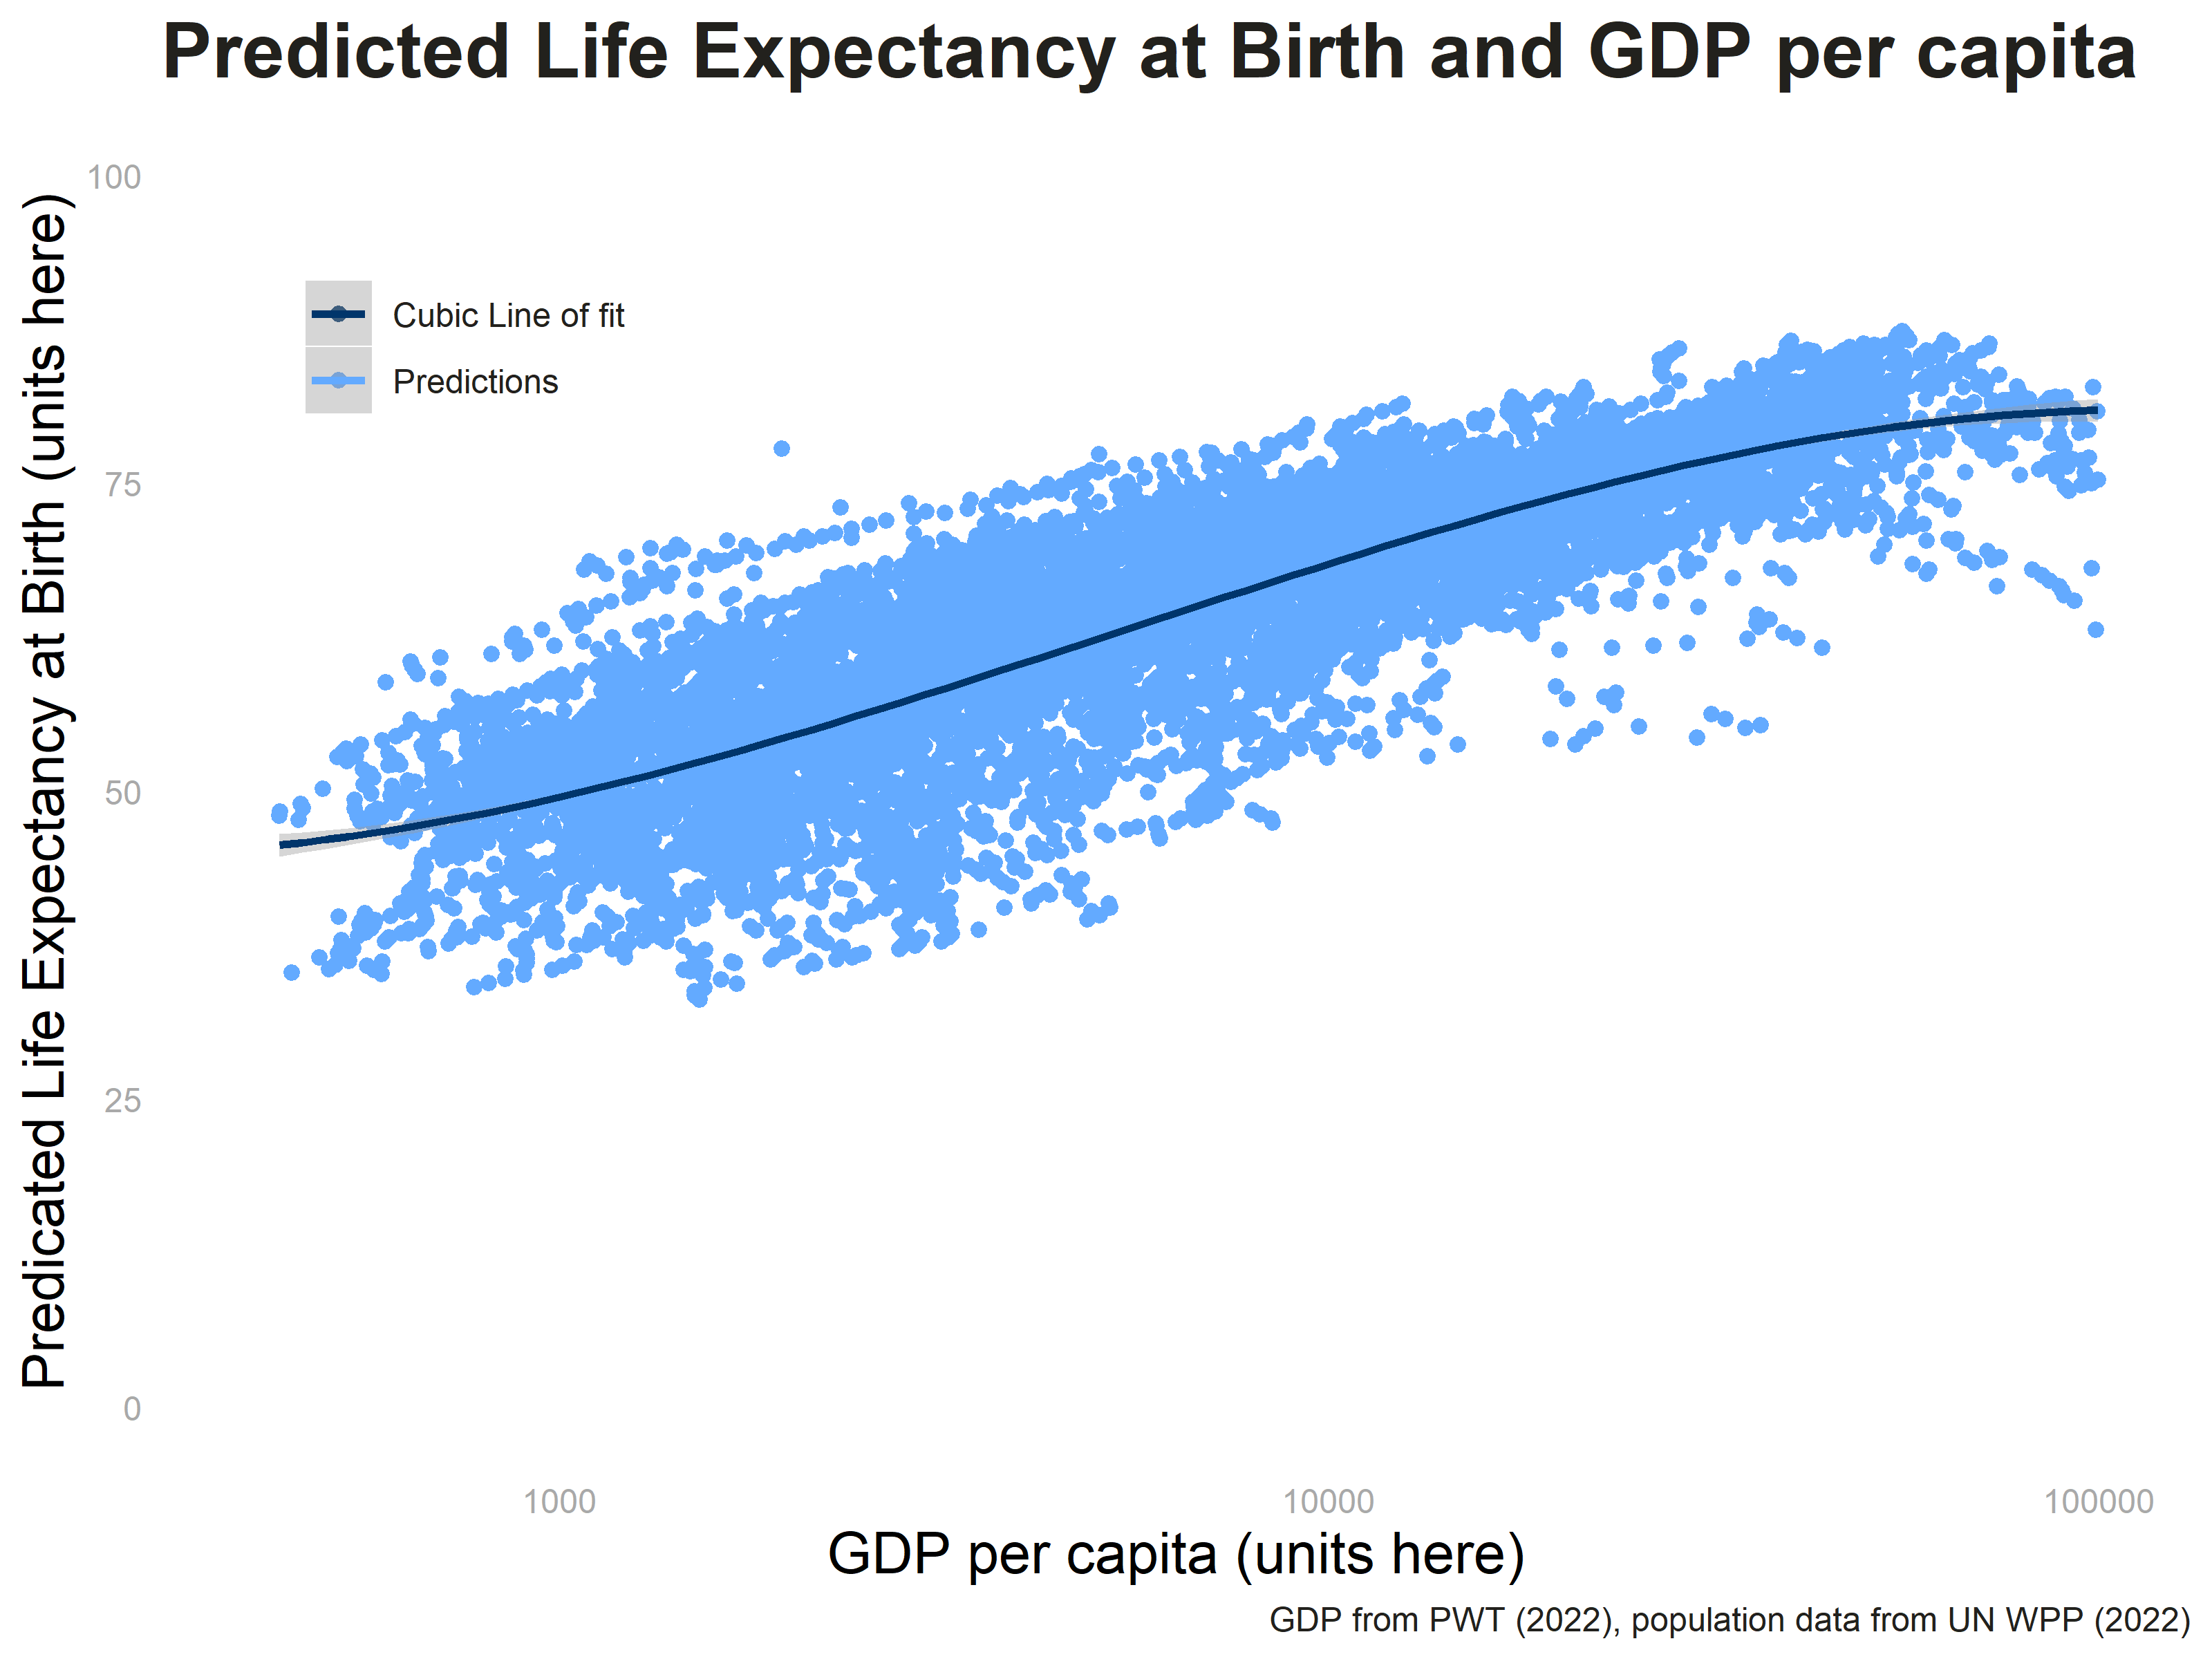
\includegraphics[width=0.8\textwidth]{figures/ECON-412/gdp_pc_le_predictions.png}
        \caption{Block diagram of a 1st order system.}
    \end{figure}      
    \end{column}
% create the column with the second image, that also
% occupies half of the slide
    \begin{column}{.5\textwidth}
    \begin{figure}
        \centering
        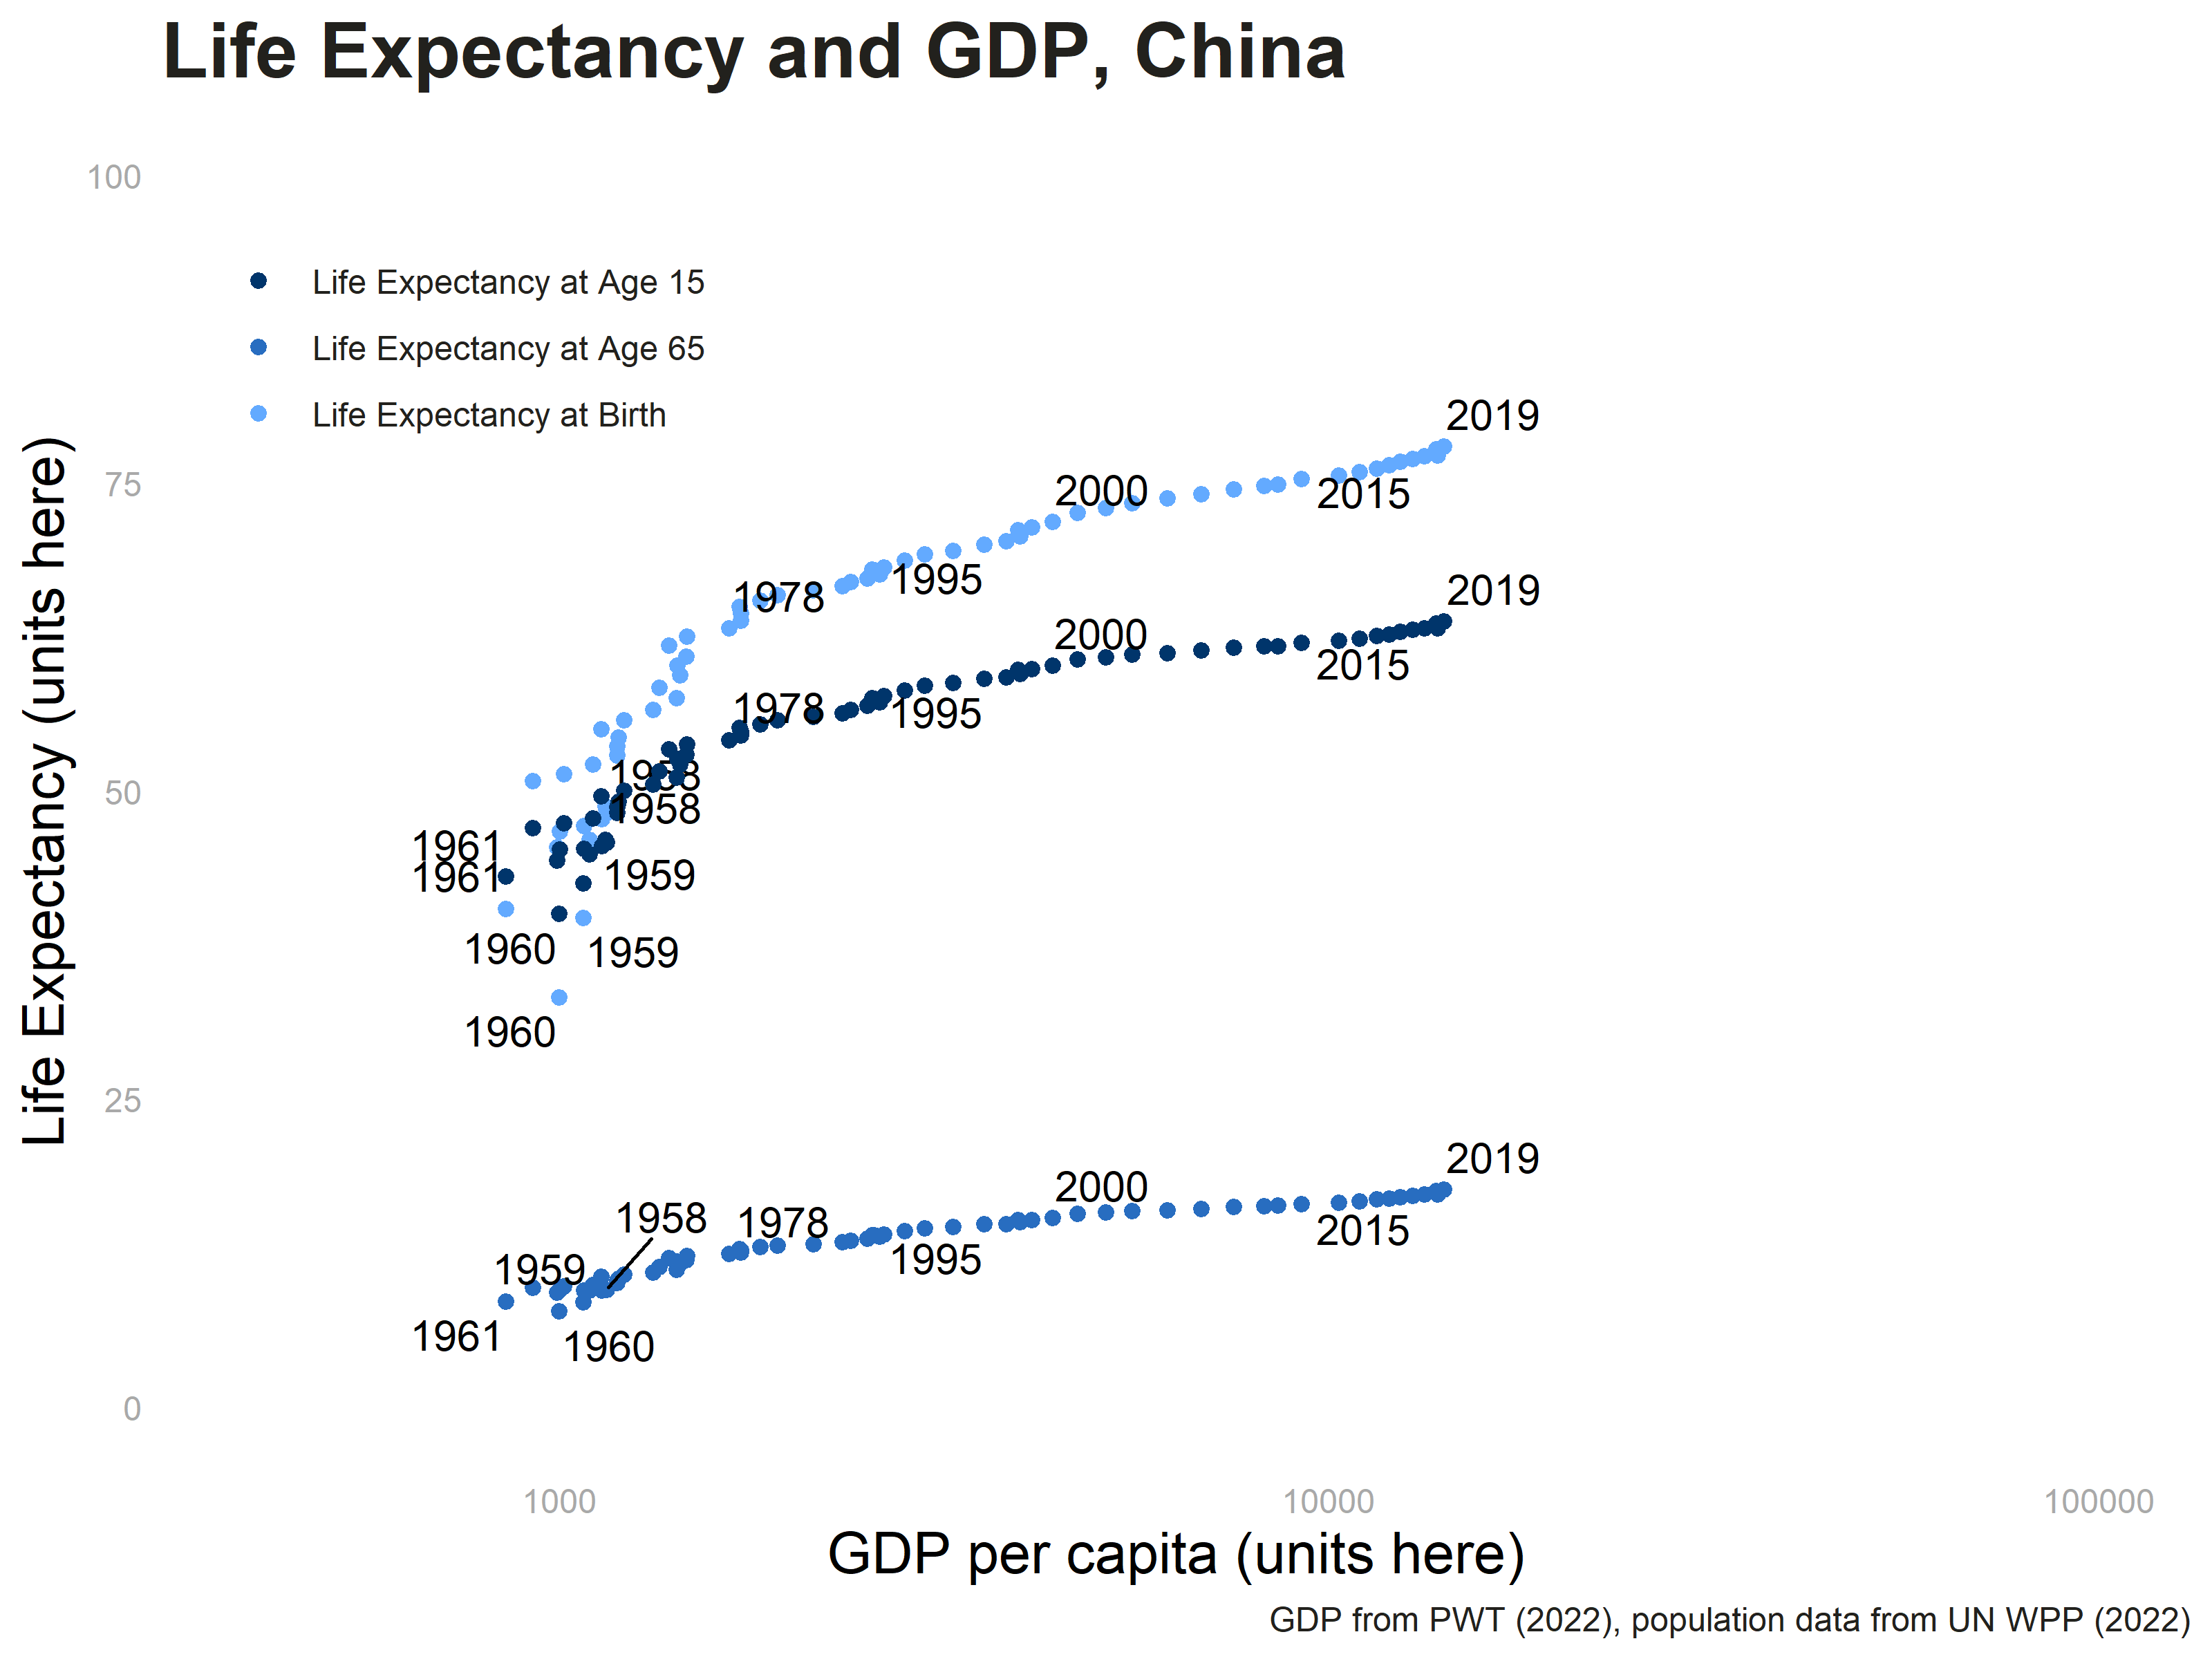
\includegraphics[width=0.9\textwidth]{figures/ECON-412/gdp_pc_le_China.png}
        \caption{Step response of a 1st order system.}
    \end{figure}
    \end{column}
\end{columns}
\end{frame}


\section{Framework}

\begin{frame}
\frametitle{An Ugly Regression Slide}
\begin{block}{Full Specification}
\begin{equation}
\begin{split}
Y_{j,t} = \beta_0 + & \beta_1 trade\_shock_{j,t} + \beta_2 positions_{j,t} + \beta_3 grain\_prices_{j,t} 
\\ & + \beta_4 non\_Han_{j,t} + \beta_7 non\_Han_{j,t} \times trade\_shock
\\ & + \beta_8 non\_Han_{j,t} \times grain\_prices + \lambda_t + \alpha_j + \epsilon_{j,t}
\end{split}
\end{equation} 
\end{block}
{\tiny
\begin{itemize}
\item $Y_{j,t}$: mortality outcome in village $j$ in time $t$\\
{\tiny $Y>1$, relatively worse for women. $Y<1$, relatively better}
\item $trade\_shock_{j,t} $: trade shock proxy
\item $grain\_prices_{j,t}$ weather proxy
\item $positions_{j,t}$ : wealth proxy
\item $non\_Han_{j,t}$ : ethnicity proxy
\item $Confucian_{j,t}$ philosophy proxy 1
\item $Buddhist_{j,t}$ : philosophy proxy 2
\item $\lambda_t$ : time trend ; $\alpha_j$ village fixed effects; $\epsilon_{j,t}$ error term 
\end{itemize}}

\end{frame}


\section{Results}


{
\setbeamertemplate{navigation symbols}{}
\begin{frame}[plain]
    \makebox[\linewidth]{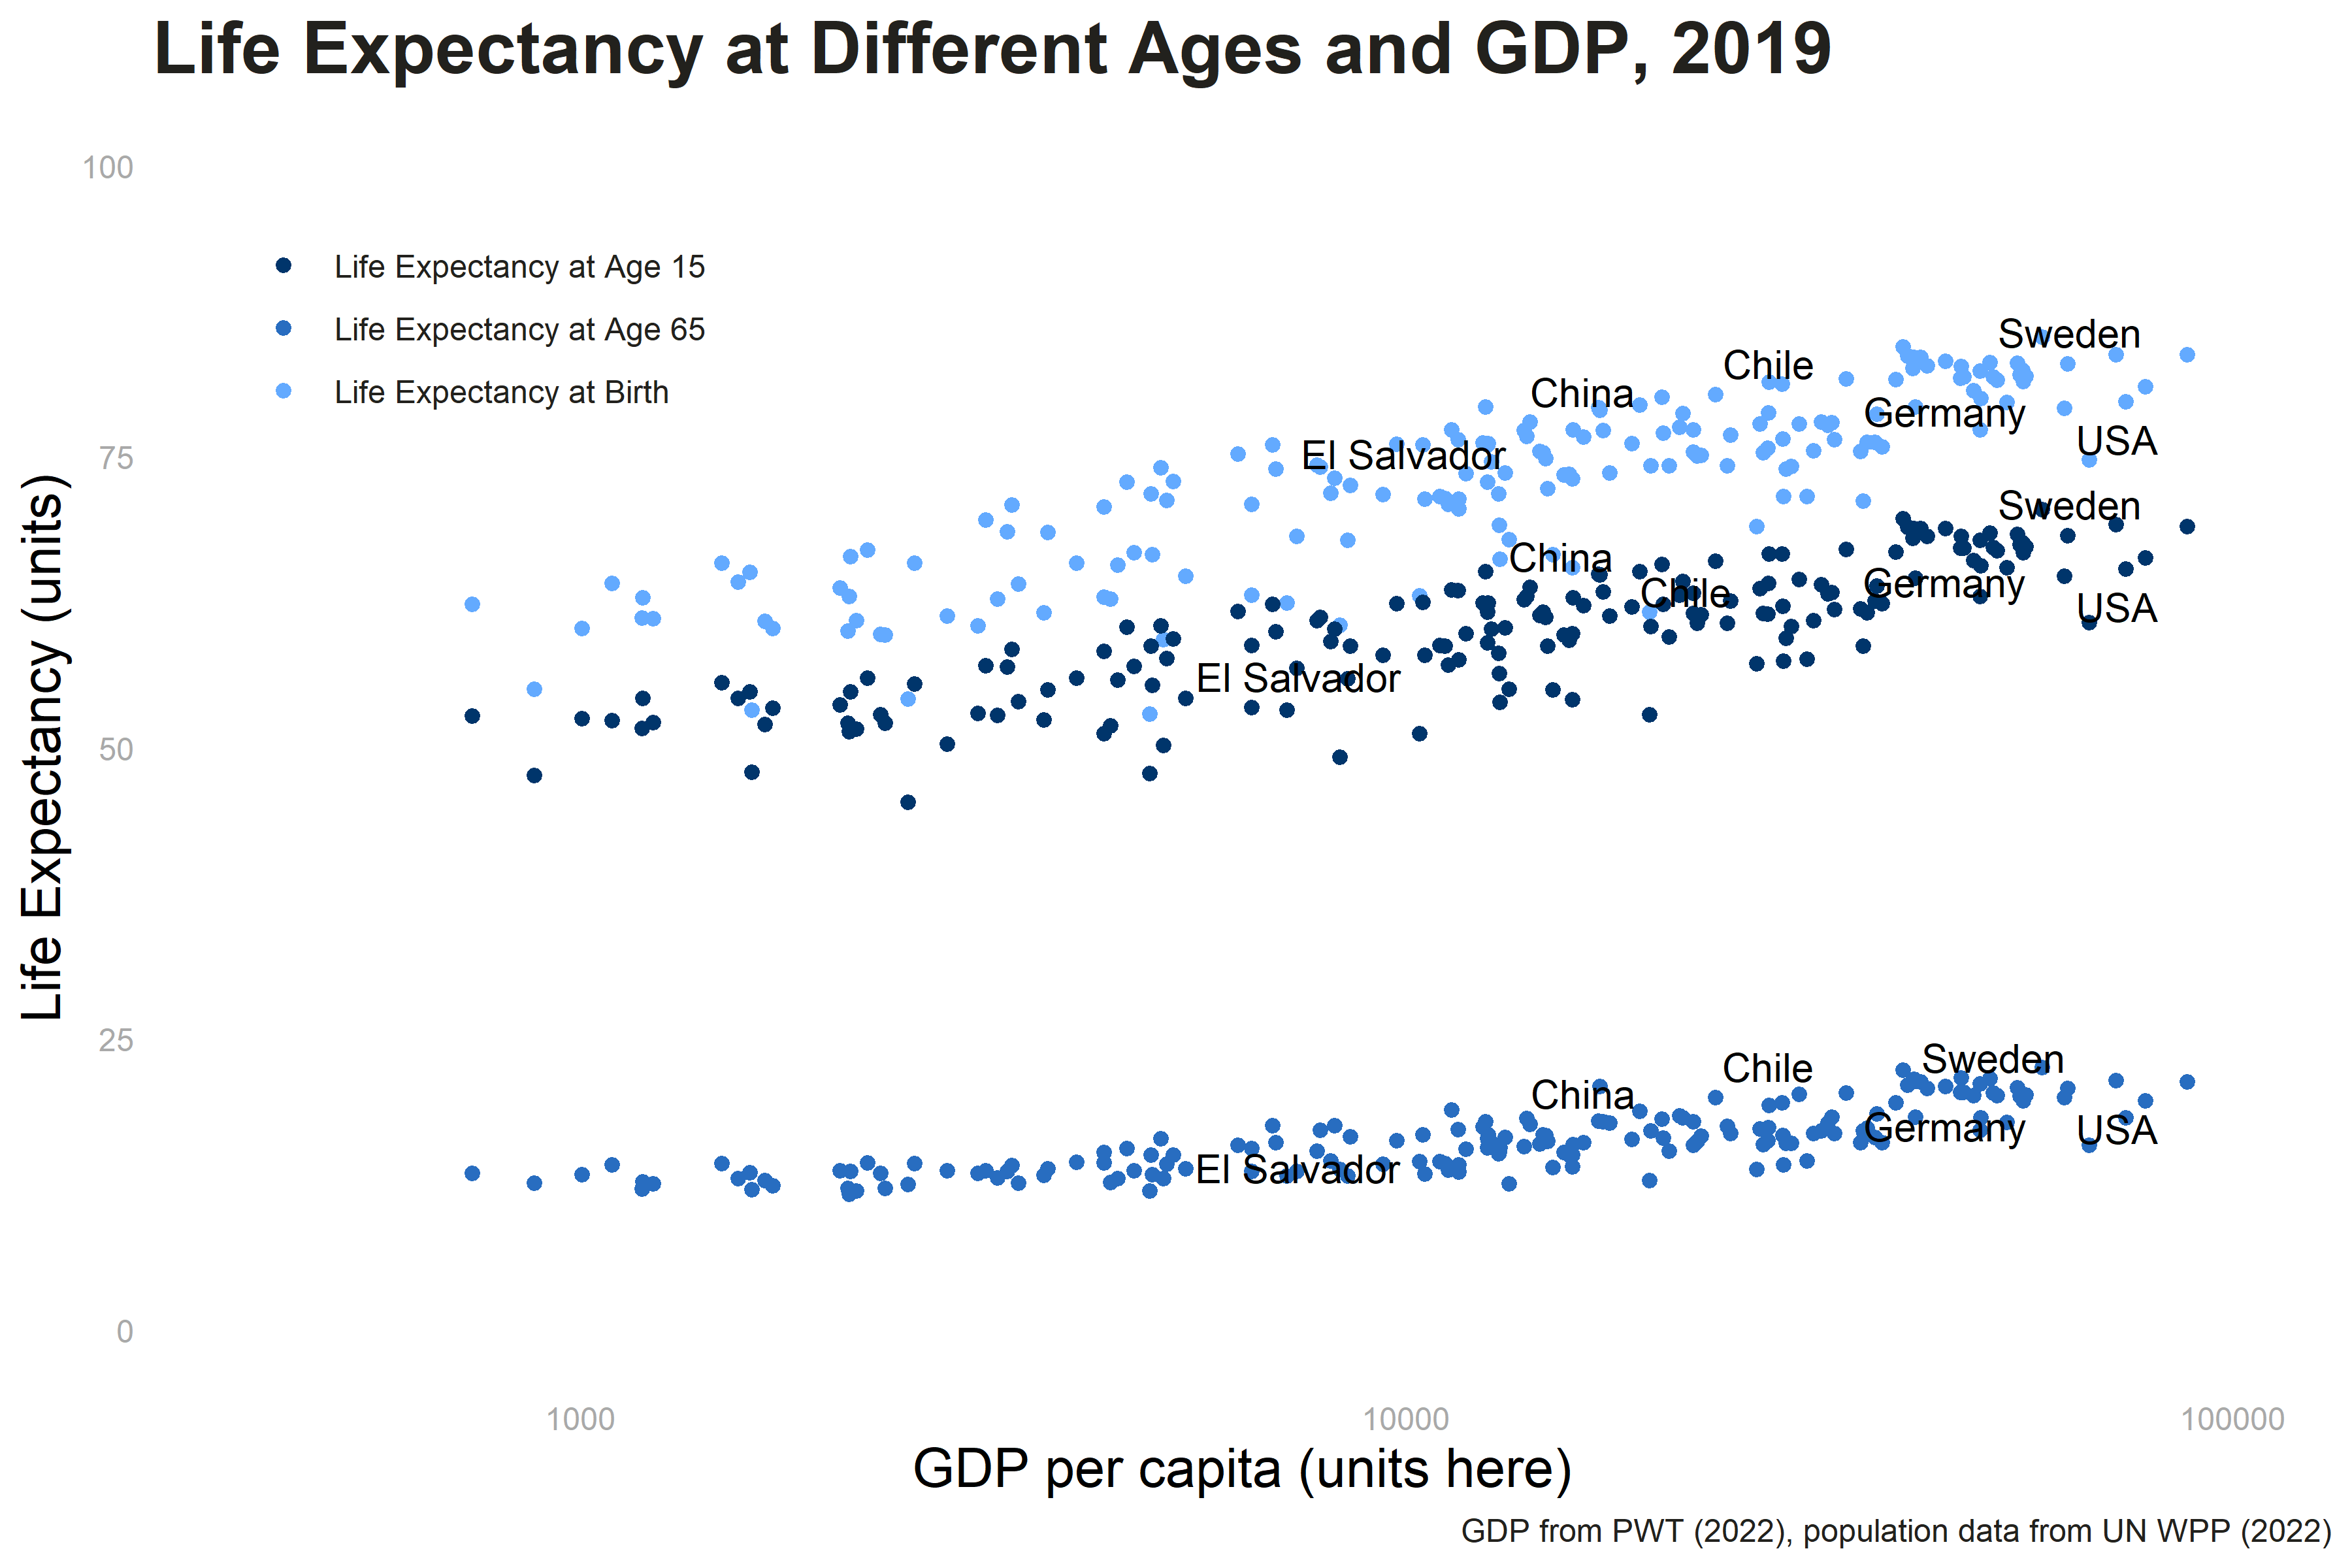
\includegraphics[width=.7\paperwidth]{figures/ECON-412/gdp_pc_le_2019.png}}
\end{frame}
}



\begin{frame}[label=target-slide]
\frametitle{Target Slide \hyperlink{source-slide}{\beamerbutton{Source Slide}}}
\begin{block}{Mortality Outcome}
\begin{equation}
Mortality \ Index = \frac{Deaths \ ratio_{females}}{ Deaths \ ratio_{males}}
\end{equation}
\end{block}

\begin{block}{Equivalently:}
\begin{equation}
Mortality Index = \frac{deaths_{t+3,females}}{present_{t,females}}\Big/\frac{deaths_{t+3,males}}{present_{t,males}} 
\end{equation}
\end{block}

For 1-20 by fives and tens, 21-50, 51-80 \emph{sui} age brackets\\
{\tiny Age in \emph{sui} = Western age + 1.5 years}
\end{frame}

\begin{frame}[label = datadefs]
\frametitle{Data Definitions}
{\tiny
\begin{itemize}
\item Outcomes given as number of female deaths in the age bracket from $t$ to $t+3$ relative to female population in the age bracket, divided by male mortality from $t$ to $t+3$ relative to male population in the same age bracket. 
\item $Y>1$ indicates greater relative female mortality.\\
\item \emph{Trade Shock} is given by the log value of exports (in log \emph{taels} of silver, where 1 \emph{tael} is about 38 grams) divided by log kilometer distance to Yingkou. Export data comes from the Chinese Maritime Customs Service, available via CMGPD 2011.\\
\item Grain prices given from the Qing dynasty grain reporting system, aggregated from the monthly to triannual level. Prices are recorded in \emph{taels} per \emph{shi} (a measure of volume for grain). Prices for Fengtian Prefecture from CMGPD, for Jinzhou prefecture from the author.
\item \emph{Position} gives the proportion of the village population that has a position in the Qing bureaucracy.\\
\item \emph{Non-Han Names} gives the proportion of the population with a non-Han name.\\
Data for \emph{Position} and \emph{Non-Han Names} are available from CMGPD 2011.\\
Temple data digitized by the author from the \emph{Fengtian Tongzhi}.\\
\item \emph{sui} age = Western age + 1.5 years, on average. \\
\item Column (1) presents regressions with the outcome variable listed in the title on just economic variables. 
\item Column(2) gives the model with $non\_Han$, controlling for background economic factors. \item Column (4) presents the same model, except exchanging $non\_Han$ with $Confucian$ and $Buddhist$, the number of Confucian and Buddhist temples within 15 km of a village, respectively. \item Columns (3) and (5) present the cultural proxies interacted with the $trade\_shock$ and $grain\_price$\\
\end{itemize}
Back to \hyperlink{results}{\beamerbutton{results}}}.
\end{frame}

\section{Summary Stats}



\begin{frame}[label = sumstats]
\frametitle{Summary Stats \hyperlink{datadefs}{\beamerbutton{Data Definitions}} }

{\tiny

\begin{table}[htbp]\centering \caption{Summary Statistics  \label{tab:sumstats}}
\begin{tabular}{l c c c c c}\hline
\multicolumn{1}{c}{\textbf{Variable}} & \textbf{Mean}
 & \textbf{Std. Dev.}& \textbf{Min.} &  \textbf{Max.} & \textbf{N}\\ \hline
1-5 Mortality Index & 0.947 & 2.305 & 0 & 23.5 & 523\\
Trade Shock & 0.319 & 0.645 & 0 & 2.529 & 523\\
Grain price & 0.68 & 0.213 & 0.288 & 1.243 & 364\\
Position & 0.02 & 0.02 & 0 & 0.179 & 523\\
Non-Han & 0.037 & 0.029 & 0 & 0.185 & 523\\
Confucian & 4.595 & 6.612 & 0 & 21 & 523\\
Buddhist & 2.778 & 5.367 & 0 & 18 & 523\\
\hline\end{tabular}
\end{table}

} % end tiny
\end{frame}


\begin{frame}[label = focexample]
\frametitle{Exercise: The Competitive Firm's Problem}

\begin{center}
Demand: $Q = 10 - 2P \iff \textcolor{PineGreen}{P = 5 - \frac{1}{2}Q}$\\
Total Cost: $\textcolor{NavyBlue}{C(Q) = 2Q + Q^2}$
\end{center}
What will be the equilibrium price and quantity for a competitive (price-taking) firm?
\begin{equation*}
\begin{split}
\max_{Q} & \textcolor{BrickRed}{P}Q - \textcolor{NavyBlue}{C(Q)}\\
\max_{Q} & \textcolor{BrickRed}{P}Q - (\textcolor{NavyBlue}{2Q+Q^2})
\end{split}
\end{equation*}

Taking the derivative of the objective function (the thing we're maximizing) with respect to $Q$, we obtain our FOC:
\pause
\begin{equation*}
\begin{split}
\text{FOC}: P& = MC\\
\Rightarrow \textcolor{PineGreen}{5 - \frac{1}{2} Q} & = 2 + 2Q\\
\Rightarrow Q^* = 1.2; & P^* = 4.4
\end{split}
\end{equation*}

\end{frame}

\begin{frame}{A really padded table}
\centering
\begin{tabular}{lccc}
    Name & Exam 1 & Exam 2 & Global \\
\hline\hline
    Alice & 8.0 & 9.0 & 8.5 \\
    Bob & 9.0 & 9.8 & 9.4 \\
\end{tabular}
\end{frame}